\documentclass{beamer}
\usepackage{amsmath}
\usepackage{amssymb}
\usepackage{bm}
\usepackage{amsthm}
\usepackage{enumerate}
\usepackage{tikz-qtree}
\usepackage{soul}
\usepackage[utf8]{inputenc}

\tikzset{every tree node/.style={minimum width=2em,draw,circle},
         blank/.style={draw=none},
         edge from parent/.style=
         {draw,edge from parent path={(\tikzparentnode) -- (\tikzchildnode)}},
         level distance=1.5cm}

\usetheme{Madrid}


%Information to be included in the title page:
\title{Branching, bounding, and you!}
\author{Joseph Diaz}
\institute{San Diego State University}
\date{December 2020}



\begin{document}

\frame{\titlepage}

\begin{frame}
\frametitle{Introduction - When enumerating isn't good enough}
In many combinatorial and discrete optimizations problems it is possible, at least in principle,
to come up with a means of generating all possible states of a problems and checking for
which represents the best solution. \vfill
In practice, however, this is usually impossible. As these states could be so 
\textit{numerous} that it would take far too long to generate and check each, and very likely 
there isn't enough space in any computer's RAM to store them all.\vfill
These 2 issues taken together lead to the development of...
\end{frame}

\begin{frame}
\frametitle{Introduction - Branch and Bound!}
What even \textit{is} it, though?
\begin{block}{Answer}
Branch and Bound is an algorithm design paradigm with applications in Discrete Optimization and
Combinatorial Optimization in which the following are employed
\begin{itemize}
    \item A set of possible solutions is generated by a state space search.
    \item A means of recursively splitting the solution set into subsets.
    \item A method for determining if any of these subsets has a viable solution, or if it 
    should be cut from the search space. 
\end{itemize}
\end{block}
\end{frame}

\begin{frame}
\frametitle{Method - Branching}
\begin{columns}
    \column{.5\textwidth}
    This set $S_1$ of possibles solutions, and its subsets, are usually represesented as a 
    binary tree; where $S_1$ is the root and each pair of child nodes are disjoint subsets of 
    the parent they belong to. So in general, the relationship between $S_1$ and the other nodes 
    is the following recursive relation:
    $$\forall i \in \mathbb{N}, S_i = S_{2i} \cup S_{2i+1},
    S_{2i} \cap S_{2i+1} = \varnothing$$

    \column{.5\textwidth}
    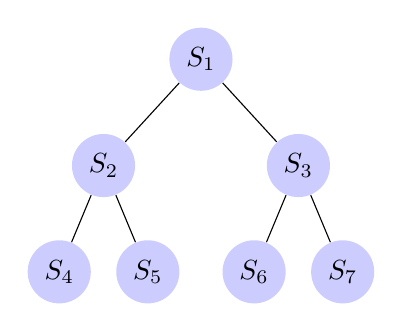
\begin{tikzpicture}  
        [scale=.9,auto=center,every node/.style={circle,fill=blue!20}] 
        % here, node/.style is the style pre-defined, that will be the default layout of all the nodes. You can also create different forms for different nodes.  
          
        \node (a1) at (0,0) {$S_1$};
        \node (a2) at (-1.375,-1.5) {$S_2$};
        \node (a3) at (1.375,-1.5) {$S_3$};
        \node (a4) at (-2,-3) {$S_4$};
        \node (a5) at (-.75,-3) {$S_5$};
        \node (a6) at (.75,-3) {$S_6$};
        \node (a7) at (2,-3) {$S_7$};
        
        
        \draw (a1) -- (a2); % these are the straight lines from one vertex to another  
        \draw (a1) -- (a3);  
        \draw (a2) -- (a4);  
        \draw (a2) -- (a5);  
        \draw (a3) -- (a6);  
        \draw (a3) -- (a7);  
        
      \end{tikzpicture}
\end{columns}
\end{frame}


\begin{frame}
\frametitle{Method - Branching to Bounding}
This splitting of the solution set and tree representation is what 
gives us the ``branching'', but where does the bounding come in? \vfill
Instead of following each branch down to a leaf and comparing these solutions, we 
employ a schema to determine which branches are worth traversing and which aren't.
\end{frame}

\begin{frame}
\frametitle{Methods - Bounding}
Most Branch and Bound algorithms rely on 2 different bounds that computed using each node 
of tree:\vfill
\textbf{Optimistic Bound} - The lower (or upper, if you're maximizing) bound of all possible 
solutions represented by a given node. A quick, efficient, and accurate calculation of this 
bound is crucial if you're expecting your algorithm to get anywhere.\vfill
\textbf{Pessimistic Bound} - The best solution to the optimization problem so far. Comparison 
between this and the optimistic bound on newly visited node is the primary decision maker for
disregarding a branch or exploring it further. 
\end{frame}

\begin{frame}
\frametitle{Methods - ``Give me pseudo code''}
\begin{block}{The algorithm - In a nut shell}
Given an objective function $f(x)$ for $x \in \Omega$ and $S_1 \subset \Omega$ a set
of possible solutions. \\
\begin{itemize}
    \item[1.] Using a heuristic, locate a solution $x_h$ and store $S = f(x_h)$ or 
    $S= \infty$ if no such $x_h$ exists. $S$ will also denote best solutions found
    so far, and will serve as the pessimistic bound to compare future solutions to.
    \item[2.] Initialize a data structure of nodes representing sets of possible solutions.
    \item[3.] Take a node $S_i$ from the data structure.
    \begin{itemize}
        \item If it represents a single solution $x$
        and $f(x) < S$, store $S = f(x)$.
        \item Otherwise, branch on $S_i$ to obtain $S_{2i}$ and $S_{2i+1}$.
        \begin{itemize}
            \item If the optimistic bound on either node is greater than $S$, discard that node.
            \item Otherwise, store the node in the data structure.
        \end{itemize}
    \end{itemize}
    \item[4.] Repeat 3 until the data structure is empty.
\end{itemize}
\end{block}
\end{frame}

\begin{frame}
\frametitle{Methods - Data Structure Choice}
Choice of Data Structure can impact the utility and ``behavior'' of the algorithms itself:
\begin{itemize}
    \item Queue - Yields behavior similar to a ``breadth first'' search. As in, all nodes 
    on a given level are examined before going down a branch.
    \item Stack - Yields behavior similar to a ``depth first'' search, where-in each branch is 
    explored to it's exhaustion before examining other nodes.
    \item Priority Queue - If each node is sorted by it's bound, then this structure gives 
    a ``best first'' sort of search where the most promising branches are explored first.
\end{itemize}
\end{frame}

\begin{frame}
\frametitle{Problem 1 - The Knapsack problem}
The Knapsack problem, a problem of resource allocation with applications in economics, 
has been a popular toy problem to solve using Branch and Bound. The problem is thus:
\begin{block}{"What should I take?"}
Given a collection of items, each with a weight and a value; which items should you take such
that the overall value of the items taken is maximized, subject to the maximum weight that you 
can carry in your knapsack?
\end{block}
The problem itself is very old, but the name is often attributed to the American Mathematician
Tobias Dantzig.
\end{frame}

\begin{frame}
\frametitle{Problem 1 - Results}
    \begin{figure}
    \centering
    \includegraphics[width=\linewidth]
    {BnBalone.jpg}
    \end{figure}
\end{frame}

\begin{frame}
\frametitle{Problem 1 - Results}
    \begin{figure}
    \centering
    \includegraphics[width=\linewidth]
    {ForceVsBound.jpg}
    \end{figure}
\end{frame}

\begin{frame}
\frametitle{Problem 2 - What's minimizer of the Rosenbrock function?}
While developed with discrete optimization in mind, Branch and Bound can also be implemented 
on more general Numerical optimization (Like what we do in class). \vfill
Bounding functions of multiple continuous variables over arbitrary intervals/regions 
is not trivial, but can be accomplished using interval arithmetic. Using this sort of schema, 
we can adapt branch and bound 

\end{frame}

\begin{frame}
\frametitle{Problem 2 - Results}
\begin{center}
\LARGE{ERROR 404 - Page Not Found}    
\end{center}
\end{frame}

\begin{frame}
\frametitle{Conclusions}
Branch and Bound is the most common algorithm paradigm in use for solve NP-Hard optimization
problems; like the Travelling Salesmen Problem for example. Indeed, some generalizations of the 
algorithm effectively subsume other well known search algorithms like A$^*$ and B$^*$.
\end{frame}

\begin{frame}
\frametitle{The End}
\begin{center}
\LARGE{\st{Rebukes?}}\vfill
\LARGE{\st{Compliments?}}\vfill
\LARGE{Questions?}
\end{center}
\end{frame}

\end{document}